\chapter{Application Analysis} \label{ch:appanalysis}
This chapter will explore the application domain from the A$^3$ model. First the basic principles of stereo vision will be described and then other aspects such as color versus grayscale etc. are analyzed. The results from this chapter will be used in the next chapter \vref{ch:req}.

\section{The Basic Principal of Stereo Vision}\label{sec:basicstereo}
A standard stereo vision setup consist of two similar cameras placed horizontally at a specified distance from each other. This distance is called the baseline. Figure \vref{fig:2cams_all} shows an example of this setup.\\
\begin{figure}[ht!]
  \centering
  \begin{subfigure}[t]{1\textwidth}
    \centering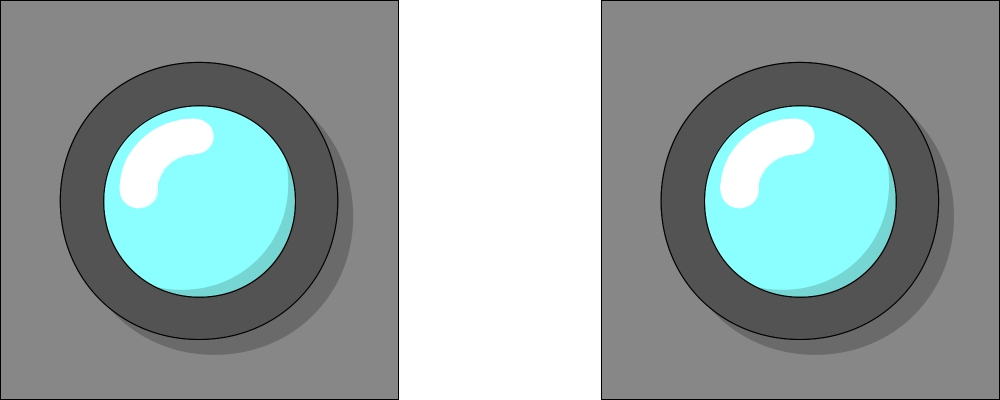
\includegraphics[width=0.4\textwidth]{figures/2cams_fro}
    \caption{Seen from the front\label{fig:2cams_fro}}
  \end{subfigure}\vspace{0.4cm}
  \begin{subfigure}[t]{1\textwidth}
    \centering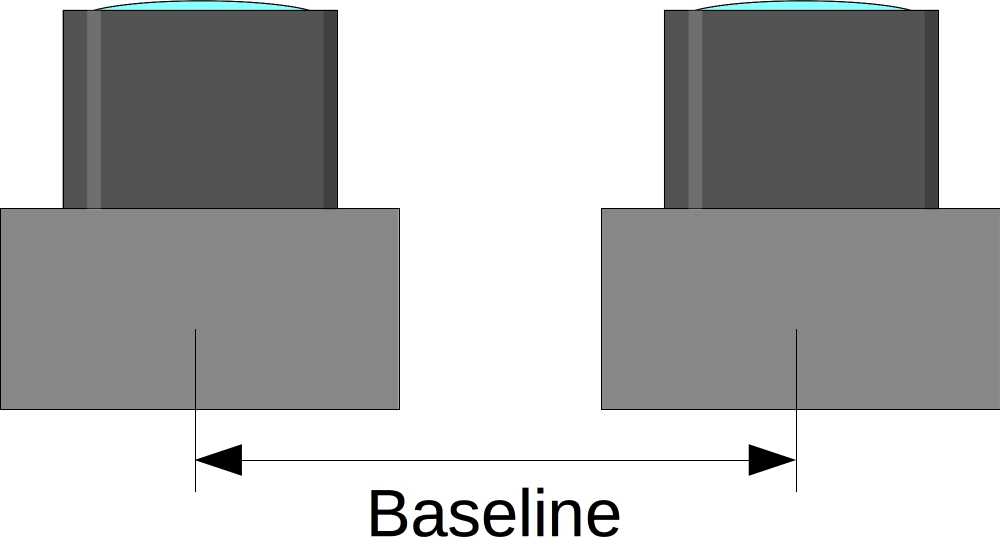
\includegraphics[width=0.4\textwidth]{figures/2cams_top}
    \caption{Seen from above\label{fig:2cams_top}}
  \end{subfigure}
  \caption{Illustration of a standard stereo setup\label{fig:2cams_all}}
\end{figure}

Figure \vref{fig:imgplane_all} shows how a scene is seen by the camera, is inverted in the optical center and projected onto the image sensor in the camera. The original image plane is located at the position of the image sensor but it is inverted compared to scene captured. To simplified comparisons to the real world an image plane can be placed opposite of the optical center at the same distance from the center and this image plane will not be inverted.

\begin{figure}[ht]
  \centering
  \begin{subfigure}[t]{0.3\textwidth}
    \centering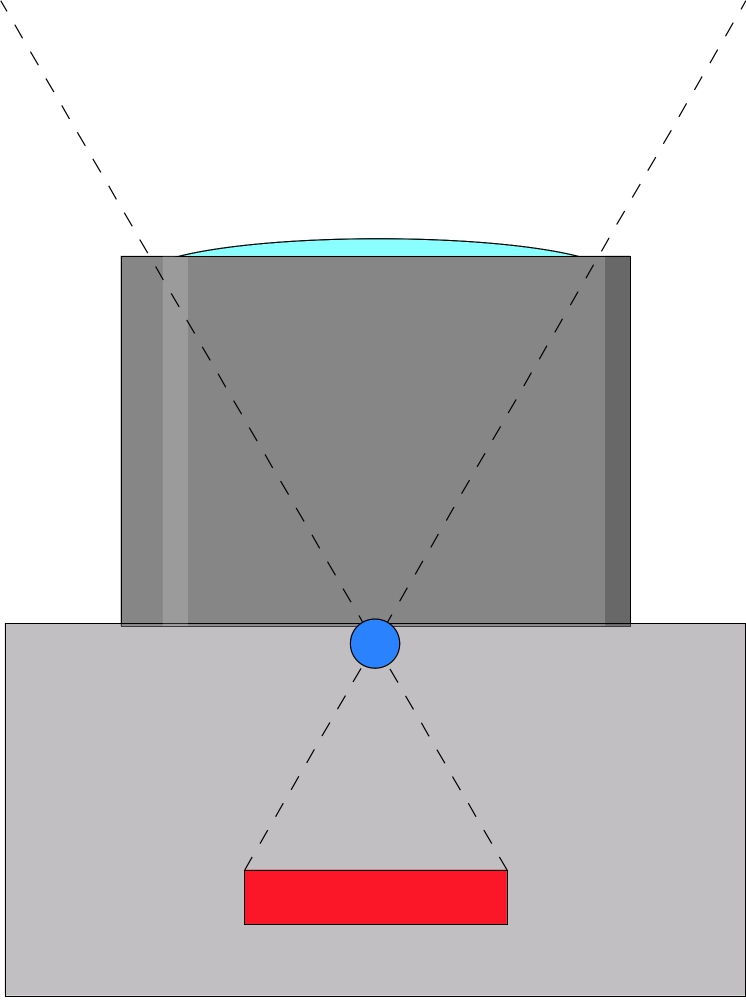
\includegraphics[height=4cm]{figures/imgplane_1.jpg}
    \caption{Location of the optical center and image sensor\label{fig:imgplane1}}
  \end{subfigure}\hspace{0.5cm}
  \begin{subfigure}[t]{0.3\textwidth}
    \centering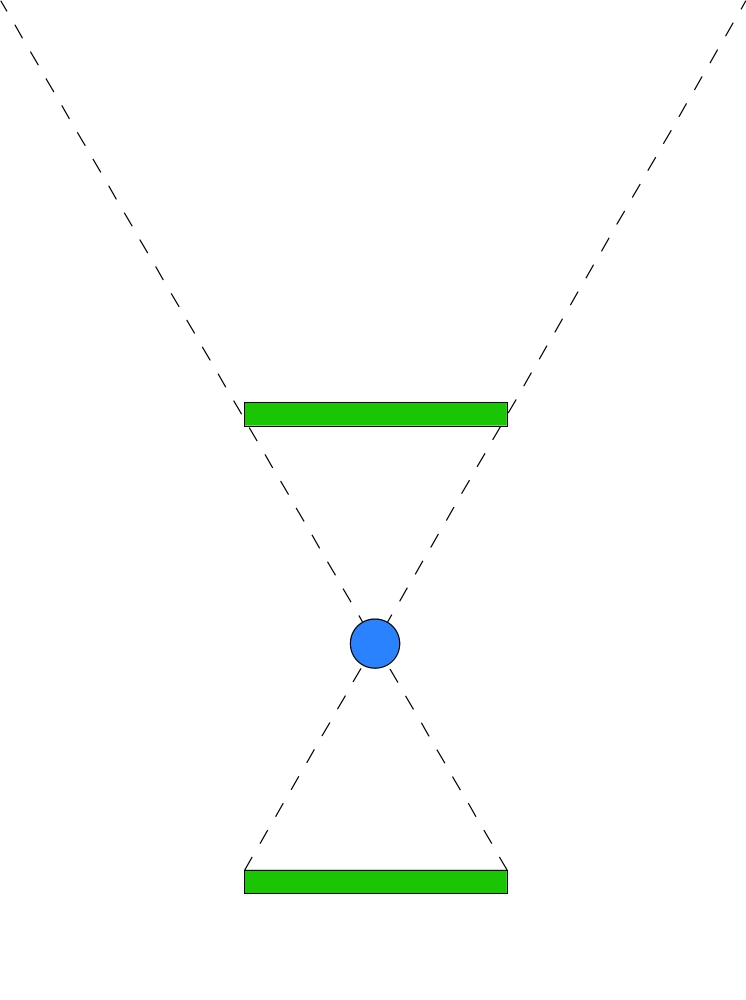
\includegraphics[height=4cm]{figures/imgplane_2}
    \caption{Location of the image plane\label{fig:imgplane2}}
  \end{subfigure}\hspace{0.5cm}
  \begin{subfigure}[t]{0.3\textwidth}
    \centering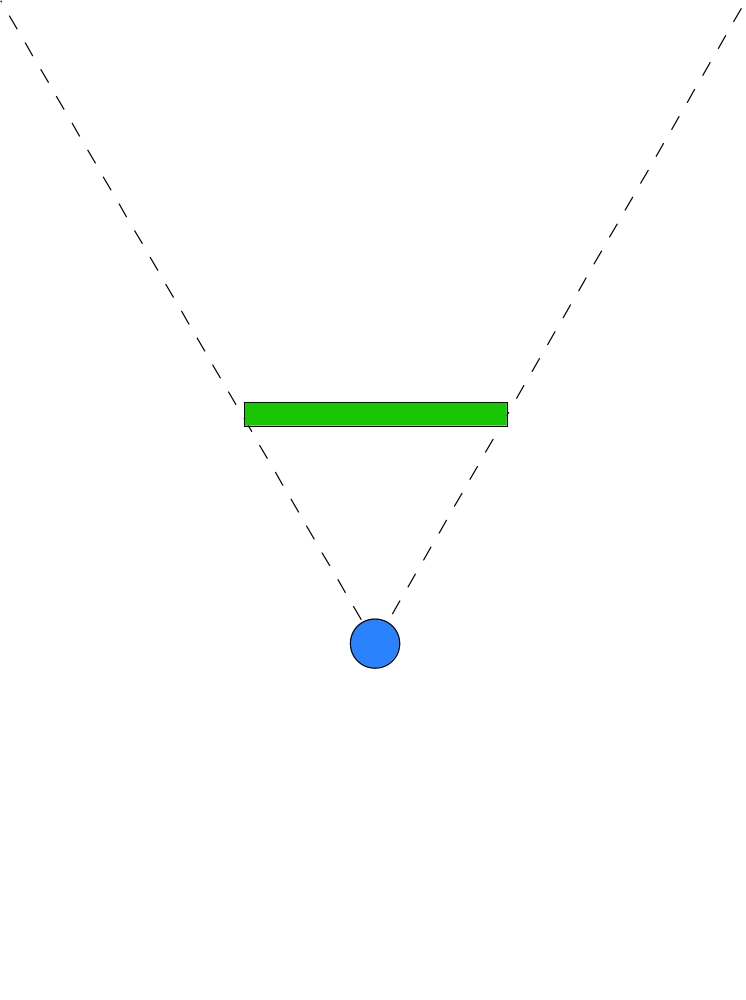
\includegraphics[height=4cm]{figures/imgplane_3}
    \caption{This illustration will be used to to explain disparity\label{fig:imgplane3}}
  \end{subfigure}
  \begin{subfigure}[t]{0.75\textwidth}
    \centering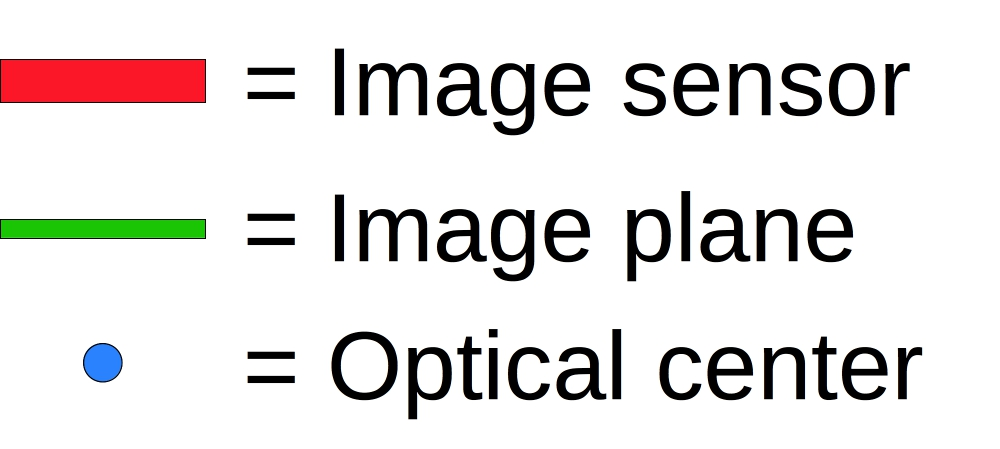
\includegraphics[width=0.4\textwidth]{figures/imgplane_legends}
  \end{subfigure}\hspace{0.5cm}
  \caption{Illustration of going from camera to image plane\label{fig:imgplane_all}}
\end{figure}

Figure \vref{fig:2points_1} shows that a single camera is not able to differentiate between two points at the same angle from the optical center but a different distance. Figure \vref{fig:2points_2} shows that adding the second camera shows that you then are able to differentiate between the two points.

\begin{figure}[ht]
  \centering
  \begin{subfigure}[t]{0.45\textwidth}
    \centering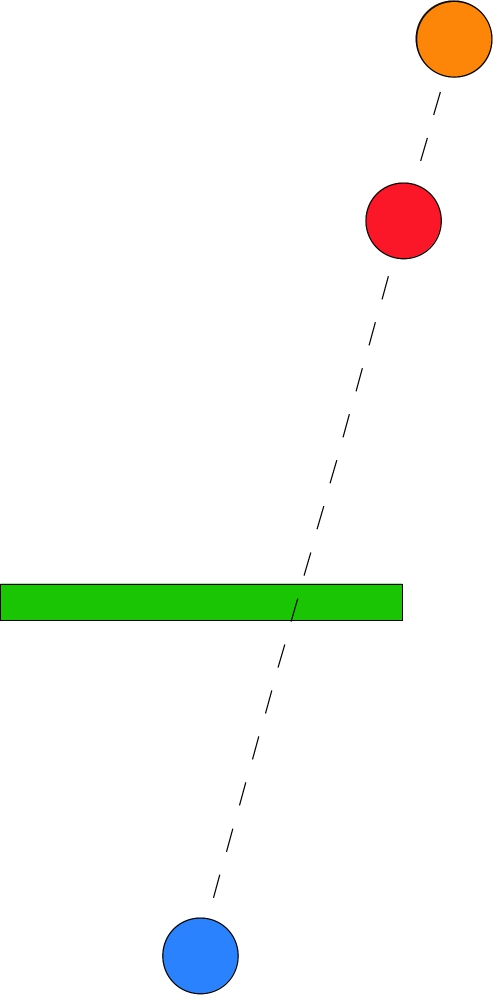
\includegraphics[height=4cm]{figures/2points_1}
    \caption{Seen from a single camera\label{fig:2points_1}}
  \end{subfigure}
  \begin{subfigure}[t]{0.45\textwidth}
    \centering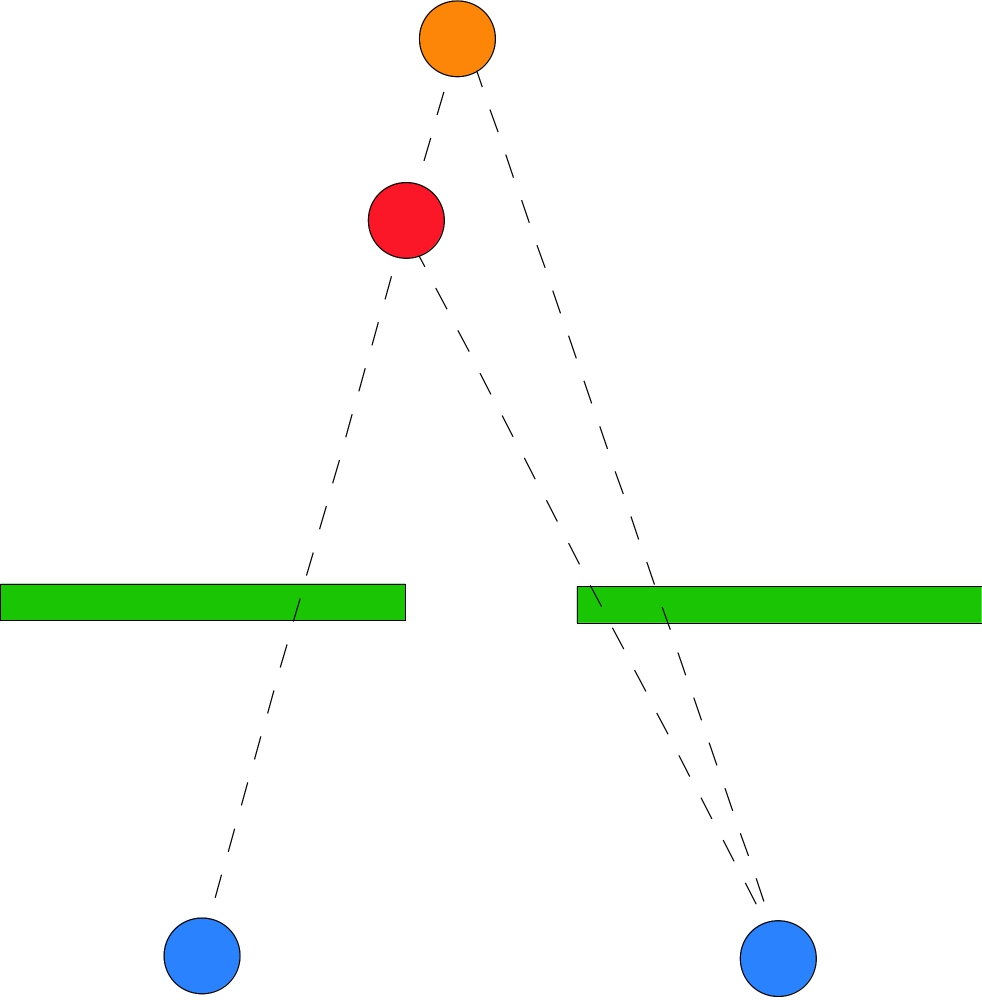
\includegraphics[height=4cm]{figures/2points_2}
    \caption{Seen from two cameras\label{fig:2points_2}}
  \end{subfigure}
  \caption{Example pf two points in a scene at different depths\label{fig:2points_all}}
\end{figure}

Figure \vref{fig:dispall} shows how the depth to a point can be calculated from the difference in x-positions on the image plane (the disparity). Figure \vref{fig:disp_long} and \vref{fig:disp_short} shows how the disparity change depending on the distance to the point. Figure \vref{fig:bfz_disp} shows the point in the scene (p), where line of sight cross the image planes (i$_1$ and i$_2$) and the optical centers (c$_1$ and c$_2$). From these points two similarly angled  triangles can be created. One between p, i$_1$ and i$_2$ and the other triangle between p, c$_1$ and c$_2$. For similarly angled triangles the ratio between the height and the bottom width is the same for each triangles and hence the following equation can be formed:
\begin{flalign}
  && \frac{b}{z} &= \frac{L}{z-f} = \frac{b-(x_1-x_2)}{z-f} && \label{eq:disp_1}
\end{flalign}
$x_1-x_2$ is also called the disparity, $d$, and equation \vref{eq:disp_1} can be simplified:
\begin{flalign}
  && &z = \frac{b \cdot f}{d} && \label{eq:disp_final}
\end{flalign}
In equation \vref{eq:disp_final} $b$ and $f$ is known hence only the disparity is needed to find $z$. So to find the distance to a point you should find the location of the point in the two images and calculate the displacement. 

\begin{figure}[ht]
  \centering
  \begin{subfigure}[t]{0.3\textwidth}
    \centering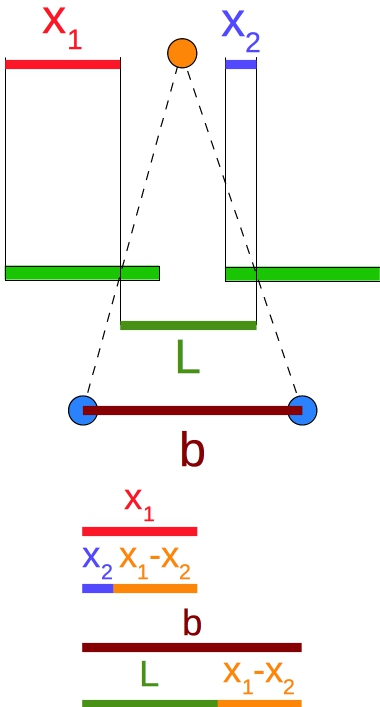
\includegraphics[height=7cm]{figures/disp_long.jpg}
    \caption{Disparity for a point far way\label{fig:disp_long}}
  \end{subfigure}\hspace{0.5cm}
  \begin{subfigure}[t]{0.3\textwidth}
    \centering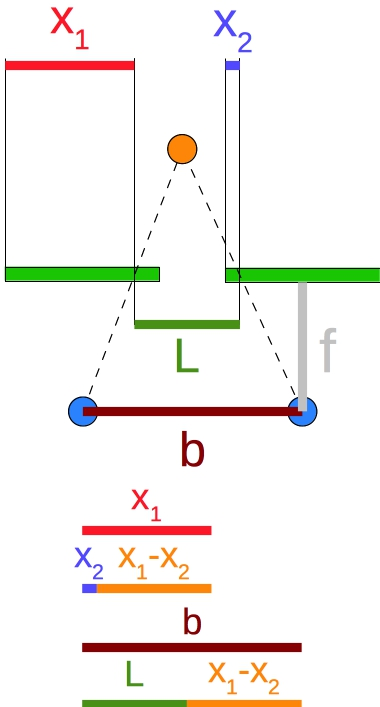
\includegraphics[height=7cm]{figures/disp_short}
    \caption{Disparity for point close\label{fig:disp_short}}
  \end{subfigure}\hspace{0.5cm}
  \begin{subfigure}[t]{0.3\textwidth}
    \centering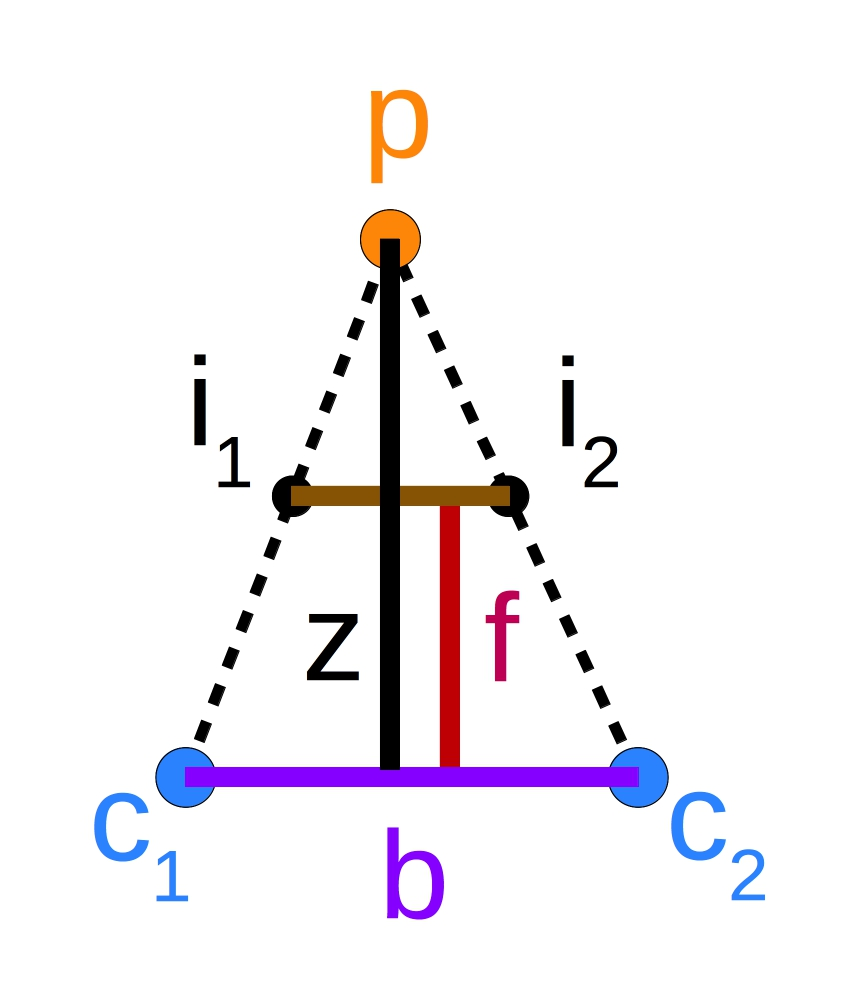
\includegraphics[height=7cm]{figures/bfz_disp}
    \caption{Illustration of triangles used for calculating the disparity\label{fig:bfz_disp}}
  \end{subfigure}
  \caption{Illustration of how to calculate depth from disparity\label{fig:dispall}}
\end{figure}

This explains the basic of stereo vision. The rest of this chapter will venture into other areals of stereo and describe the difficulties and solutions for each area.

\section{Epipolar Geometry}
Section \ref{sec:basicstereo} assumes that the stereo image planes are ideal, align exactly and being parallel with the baseline but in a real scenario the cameras will have have small imperfections and variations which will make the image planes not align perfectly.\\
 
Figure \vref{fig:nonrect} shows a pair of stereo images. As seen when searching for a corresponding point in the second camera (e.g. the top of the bottle) then a 2D search area is needed. To simplify the search epipolar geometry can be used. \\
\begin{figure}[ht!]
  \centering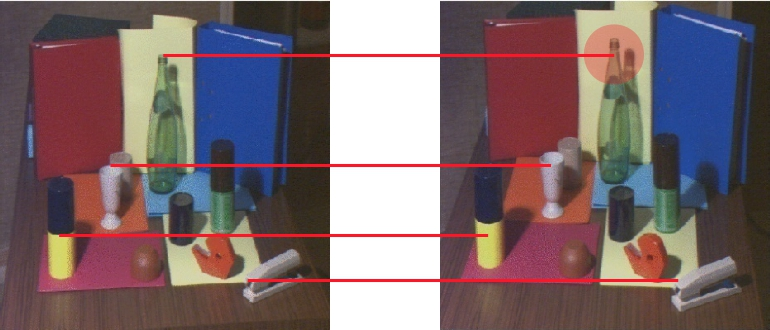
\includegraphics[height=5cm]{figures/nonrect.jpg}
  \caption{Non-rectified stereo pair\label{fig:nonrect} \cite{Mattoccia2013}}
\end{figure}

Epipolar geometry occurs when a scene is seen from two different views. Figure \vref{fig:epipolarsimple} illustrates epipolar geometry. An epipole is the projection, on one cameras image plane, of the optical center of the other camera and is illustrated on figure \vref{fig:epipolarsimple} as e$_1$ and e$_2$. The red line going through p$_1$ (the projection of point P on the image plane) and e$_1$ is called a epipolar line and a corresponding epipolar line can be found in the other image plane going through p$_2$ and e$_2$. When searching for the corresponding point in the other image the search can be simplified from a 2D search to a 1D search along the epipolar. To simplify the search further the image can be rectified.\\
\begin{figure}[ht!]
  \centering
  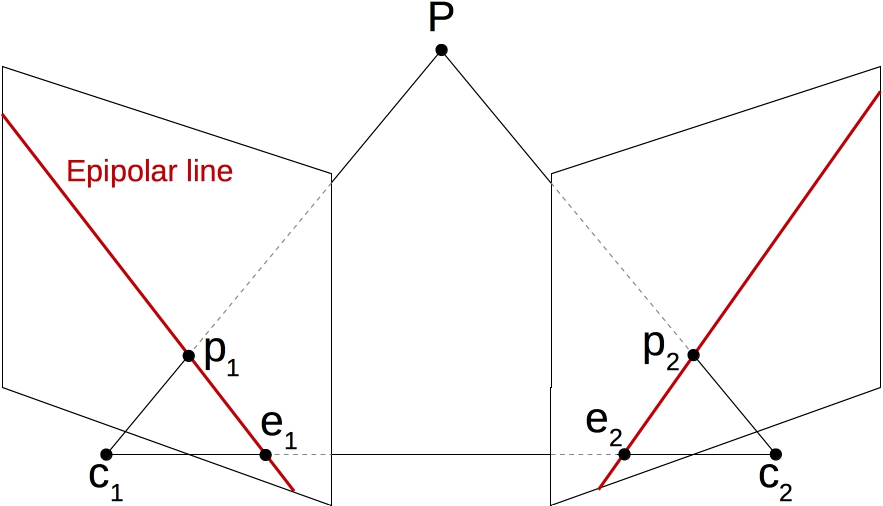
\includegraphics[height=4cm]{figures/epipolarsimple}
  \caption{Illustration of epipolar geometry}
  \label{fig:epipolarsimple}
\end{figure}

Rectification will transform the stereo images to remove lens distortion and make them into standard form. The standard form is helpful since all epipolar lines then will be horizontal and this simplifies the search for corresponding points to search along the x-axis. Figure \vref{fig:rect} shows the stereo image pair from figure \vref{fig:nonrect} but rectified. As seen, now the corresponding points can be found by following the horizontal lines or the x-axis.\\

\begin{figure}[ht!]
  \centering
  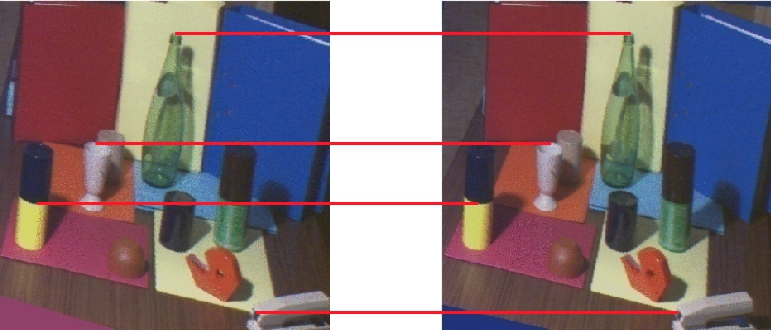
\includegraphics[height=4cm]{figures/rect}
  \caption{Rectified stereo pair\label{fig:rect} \cite{Mattoccia2013}}
\end{figure}

The issue with rectification is that it is difficult to get a perfect match with the stereo setup since the every camera and its objective will be unique and require and all new manual adjustment. HSA system theorizes that a system can be developed which instead of rectifying the image it will find the epipolar lines and feed this information to the stereo cameras.\\

In this project stereo image pairs from Middlebury Vision Test sets \cite{middlebury2016} will be used which are rectified hence the rectification of image will not be researched further in this project.

\section{Color space and gray scale}
Colors can be represented in many different ways digitally using color spaces. Two of the most common color spaces are grayscale and RGB. Some articles have researched what impact different color spaces can have on the result from a stereo algorithm.\\ 

For this project the impact of color spaces haven't been studied but instead the findings in \cite{chambon2005colour} are used. This article studies the impact of color spaces on stereo matching by investigating 9 color spaces and 3 differnet methods. Table \vref{tab:colourres} shows parts of the results from \cite{chambon2005colour}. In this table the \textit{Measure} column is the algorithm used, \textit{Type} specifies whether it is grayscale (G) or color (C) with the best color space used, the \textit{Correct} column is the percentage of correct matches and \textit{Time} is the execution time. The article conclude that using color always results in better matching but from table \vref{tab:colourres} it is notice that using grayscale lowers the execution time a lot (down to 27-51 \% of color execution time) and in most cases not resulting much worse matching results. \\
\begin{table}
  \centering
  \begin{tabular}{l r | c | c }
    Measure & Type & Correct [\%] & Time\\
    \midrule
    Ncc & G & 52.3 & 52\\
          & C & 55.2 & 141\\
    \midrule
    D$_1$ & G & 49.5 & 63\\
               & C & 51.6 & 140\\
    \midrule
    PRATT & G & 29.1 & 86\\
              & C & 45.2 & 225\\
    \midrule
    ISC & G & 44.9 & 126\\
    & C & 52.6 & 245\\
    \midrule
    SMPD$_2$ & G & 49.9 & 569\\
    & C & 56.5 & 2109 \\
  \end{tabular}
  \caption{Part of table containing results from \cite{chambon2005colour}\label{tab:colourres}}
\end{table}

Since the project mostly focus on a fast stereo matching algorithm and minding the results from table \vref{tab:colourres} it is decided to use gray scale in case Normalized Cross Correlation is used or to check whether gray scale gives much worse result of another algorithm.

\section{Resolution and disparity precision}
The depth resolution depends on different things in the stereo camera setup. The camera resolution, the focal length, the baseline etc. Looking at a equation \ref{eq:disp_final} the constraints for a camera setup can be calculated. HSA system would requires that the system have a \SI{2}{\milli\meter} depth resolution between \SI{0.5}{\meter} and \SI{1.5}{\meter} and the camera used will be a \textit{Imaging Source DMK 72BUC02}.
The range field (horopter) is what part of the system the 
\begin{flalign}
 && z &= \frac{b\cdot f}{d} && 
\end{flalign}

 

\section{Occlusions}
Occlusions occurs when a object closer to the camera setup blocks some of object or a whole object behind it. Figure \ref{fig:occlboth} illustrates two cylinders seen by a stereo camera setup where occlusion occurs. Figure \vref{fig:occltop} shows that the right camera can't see all of the blue cylinder because the red cylinder blocks the view while the left camera can see the whole of both cylinder. When searching for corresponding points in the occluded area issues occurs. Following the arrow on figure \vref{fig:occl2view} it is seen that the edge of the blue cylinder can't be found and it will result in calculating a wrong disparity value. \\

\begin{figure}[ht]
  \centering
  \begin{subfigure}[t]{0.45\textwidth}
    \centering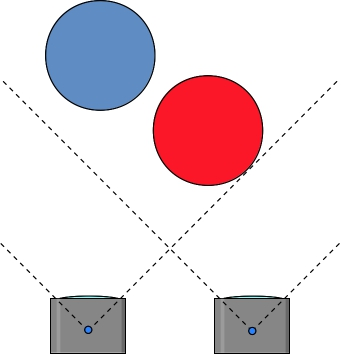
\includegraphics[scale=0.4]{figures/occltop.jpg}
    \caption{Stereo camera setup with two cylinders in the scene seen from above\label{fig:occltop}}
  \end{subfigure}\hspace{0.5cm}
  \begin{subfigure}[t]{0.45\textwidth}
    \centering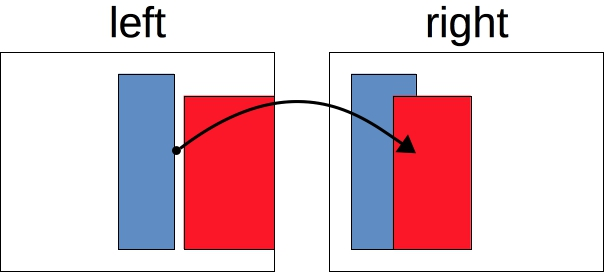
\includegraphics[scale=0.4]{figures/occl2view}
    \caption{Image seen by each camera in figure \vref{fig:occltop}\label{fig:occl2view}}
  \end{subfigure}
  \caption{Illstration of occlusions\label{fig:occlboth}}
\end{figure}

There exist different types of occlusions: partial occlusions, self occlusions, border occlusions and total occlusions. Partiel occlusions is when an object is only partial obstructed as seen on figure \vref{occlboth}. Self occlusion occurs on round surfaces such as faces, and balls and as seen on figure \vref{fig:occlself} the surfaces marked with red can be seen by one camera but not the other camera. Border occlusions occurs when an object or part of an object is outside the view of one camera but not the other camera as seen with the blue object on figure \vref{fig:occltb}. Total occlusion is when an object is completely blocked by an object in the view of one camera but not in the other camera and an example of this is seen with the red object on figure \vref{fig:occltb}.\\

\begin{figure}[ht!]
  \centering
  \begin{subfigure}[t]{0.45\textwidth}
    \centering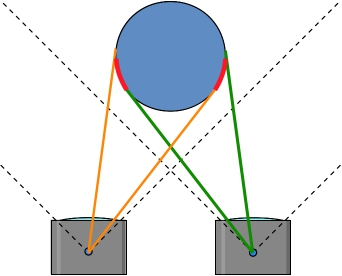
\includegraphics[scale=0.4]{figures/occlself.jpg}
    \caption{Illustartion of self occlusion seen from above\label{fig:occlself}}
  \end{subfigure}\hspace{0.5cm}
  \begin{subfigure}[t]{0.45\textwidth}
    \centering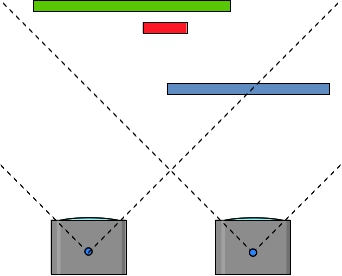
\includegraphics[scale=0.4]{figures/occltotalborder}
    \caption{Illustration of total and border occlusions seen from above\label{fig:occltb}}
  \end{subfigure}
  \caption{Illustration of different types of occlusions\label{fig:occltypes}}
\end{figure}

Occluded points can be found by running stereo matching again but switching which camera is used as reference and then compare the disparity values found for each direction. When occluded areas are found these can be filled using different methods. For this project new methods haven't been developed or studied but instead the findings from \cite{huq2013occlusion} is used which will be described in section \vrefrange{sec:nda}{sec:sls}. All these methods assume that the stereo matching is using the left image as reference i.e. the points in the left image are searched for in the right image. 

\subsection{Neighbor's Disparity Assignment : NDA}\label{sec:nda}
This is one of the simpler method to fill occlusions. It functions by selecting an occluded point, $p_L$, then find then nearest non-occluded point, $q_L$, to the left when filling non-border occlusion. With border occlusion the nearest point to the right is found instead. This method assumes that this non-occluded point is part of same surface as the occluded point (this can be seen on figure \vref{fig:occlboth}) and the disparity value from $q_L$ can be assigned to $p_L$. This method have some issues. In cases of total occlusions (see figure \vref{fig:occltb}) wrong disparity values will be given to the total occluded object since it isn't a part of the nearest surface with non-occluded points to the left. In cases with self occlusions the occluded area should have disparity values close to the disparity values of the non-occluded points to the right (This will be the area of the surface which is in view of both cameras) but using NDA will give the occluded area disparity values corresponding to the background.

\subsection{Diffusion in Intensity Space : DIS}
This method is inspired by diffusion. Diffusion is the movement of molecules or atoms from a high concentration region to a low concentration region. \\

After detecting occluded regions with cross-checking during stereo matching, the diffusion energy for the region is approximated. This method is depended on the stereo matching algorithm because it use the energy from the last iteration to determine initial diffusion energy for the area. But a change to the method can be made to make it independent from the stereo matching. The initial energy will be 0. Then the diffusion energy for non-border occlusion is found by:
\begin{equation}
E(p_L) = \min_{l_{p_L}=\{0,\dots, l_{max}\}} \left( \dfrac{1}{2 | q_L \in \mathcal{N}(p_L) \wedge l_{q_L=l_{p_L}} |} \; \sum_{q_L \in \mathcal{N}(p_L) \wedge l_{q_L = l_{p_L}}} (|\bar{I}(p_L)-\bar{I}(q_L) | + E(q_L))\right)
\end{equation}
And the diffusion energy for border occlusions are found by by:
\begin{equation}
E(p_L) = \min_{l_{p_L}=\{0,\dots, l_{p_{Lf}}-2\}} \left( \dfrac{1}{2 | q_L \in \mathcal{N}(p_L) \wedge l_{q_L=l_{p_L}} |} \; \sum_{q_L \in \mathcal{N}(p_L) \wedge l_{q_L = l_{p_L}}} (|\bar{I}(p_L)-\bar{I}(q_L) | + E(q_L))\right)
\end{equation}
The diffusion energy will be calculated for each occluded point and for each point the disparity which corresponds the minimum $E(p_L)$ is set as the disparity $l_{p_L}$ for the occluded point.

\subsection{Weighted Least Squares : WLS}
In this approach, WLS, all the non-occluded and filled occluded neighbors in a neighborhood around the occluded point is considered valid points and is used as control points in interpolation.\\
Since the neighborhood contains both foreground points and background points and the occluded point is expected to be a part of the background then the background points should have more influence than foreground points. It is assumed that the color intensity between objects is significantly different and this property can be used to distinguish between foreground points and background points. \\
Each error term in the aggregated residual should be weighted so the foreground don't have much influence. With this the aggregated residual is defined as:
\begin{equation}
  \Delta = \sum_{q_L \in \mathcal{N}(p_L)} w_{q_L} (\hat{l}_{p_L}(p_L)-l_{p_L}(q_L))^2
\end{equation}
where $w_{q_L} = e^{-\mu_L | \bar{I}(p_L) - I(q_L)|}$ (the weight) is the likelihood of $p_L$ with $q_L$ under the assumption of an exponential distribution model of $| \bar{I}_(p_L)- I(q_L) |$. $\bar{I}(p_L)$ is the mean intensity of $p_L$ and $\mu_L$ is the decay rate. $\hat{l}_{p_L}(p_L)$ is the estimated disparity of $p_L$ (will be estimated during interpolation) and $l_{p_L}(q_L)$ is the disparity of $q_L$. \\
How to estimate $\bar{I}(p_L)$ and $\mu_L$:\\
$\bar{I}(p_L)$ is the mean intensity of $p_L$ which can be obtained using mean shift algorithm in a window around $p_L$. To estimate this value the initialize the algorithm with $\bar{I}(p_L) $ equal to the intensity of $p_L$ then the mean shift algorithm repeatedly picks those neighbors inside the window that satisfy $| \bar{I}(p_L) - I (q_L) | \geq 3\mu^{-1}$ and the assign the average of intensities of the selected neighbors to $\bar{I}(p_L)$ until $\bar{I}(p_L)$ converges to a fixed average. $|\bar{I}(p_L) - I(q_L)|$ has decay rate $\mu_L$ which is related to the decay rate $\mu$ of the variable $|I(p_L) - I(q_L)|$ by $\mu_L^2 = \mu$.\\
A matrix containing all the coordinates:
\begin{equation}
F = \begin{bmatrix}
  x_1 & y_1 & 1 \\
  \vdots & \ddots & \vdots\\
  x_n & y_n & 1
\end{bmatrix}
\end{equation}
Vector with the corresponding labels for the coordinates in $F$:
\begin{equation}
L = [l_1 \; \cdots \; l_N]
\end{equation}
Linear model:
\begin{equation}
l_{p_L} = a + b x (p_L) + c y (p_L)
\end{equation}
Where $(x(p_L),y(p_L))$ is the coordinates of $p_L$ and $a$, $b$ and $c$ are the model parameters. \\
The weights for the control points can be express in a vector as:
\begin{equation}
w = [w_{q_{L1}} \; w_{q_{L2}} \; \cdots \; w_{q_{LN}}]'
\end{equation}
Then we compute two new matrices, $F_w$ and $L_w$:
\begin{flalign}
&& F_w &= diag(w)F && \\
&& L_w &= diga(w)L &&
\end{flalign}
The model parameter vector:
\begin{equation}\label{eq:parvec}
P = [\, a \; b \; c \,]'
\end{equation}
By combining the equations above then the following equation is given:
\begin{equation}
P = (F^T_wF_w)^{-1}F^T_wL_w
\end{equation}
With these equation the disparity of the occluded point can be estimated:
\begin{equation}
\hat{l}_{p_L} = [1 \; x(p_L) \; y(p_L)] P
\end{equation}

\subsection{Segmentation-based Least Squares : SLS}\label{sec:sls}
Biggest difference between WLS and SLS is that SLS only uses non-occluded points as control points. The control points is a subset of the non-occluded neighboring points. The control points are segmented from the neighborhood by applying different constraints: visibility constraint, disparity gradient constraint and color similarity cues. \\
Sequence of operations:
\begin{itemize}
\item Select an occluded point
\item Select control points from the neighborhood around the occluded point
\item Interpolate the disparity of the occluded point from the segmented control points
\end{itemize}
$\mathcal{N}(p_L)$ is a set of non-occluded, neighboring points which will be use for control points in the interpolation. For points to be added to $\mathcal{N}$ then it needs to fulfill some constraints.\\
\textbf{Disparity gradient constraint:} In most cases the horizontal closest non-occluded point to the right, $p_{Lf}$, will be part of the foreground and the occluded should be a part of the background. In this cases every non-occluded point with a lower disparity than $p_{Lf}$ will be added to $\mathcal{N}$ hence the condition for added the point, $q_L$, will be $l_{q_L} < l_{p_{Lf}}$. If the foreground object is narrow then all the non-occluded neighboring points might be from the background and have the same disparity. Due to this a second condition have to be added to the constraint. The horizontal closest non-occluded point to the left will be called $p_{Lb}$ and a second condition is created: $| l_{p_{Lb}} - l_{q_L} | \leq 1$. When these conditions are combined the constraint can be defined as:
\begin{equation}
| l_{p_{Lb}} - l_{q_L} | \leq 1 \vee  l_{q_L} < l_{p_{Lf}}
\end{equation}
\textbf{surface constraint:} It is assumed that $\mathcal{N}(p_L)$ will contain points from maximum 2 different surfaces (due to the small neighborhood). Some cases might contain a third surface but this is expected to occur very seldom and therefore it is disregarded. The point with the lowest disparity, $l_{min}$, is assumed to belong to one of the surfaces and the point with the highest disparity, $l_{max}$, is assumed to belong to the other surfaces. If $l_{max} - l_{min} \leq 1$ then it is assumed the all the points in $\mathcal{N}$ belongs to a single surfaces otherwise the points have to be segmented into 2 groups. The first group will contain all points which satisfies $| l-{max} - l_{q_L} | \leq 1$ and the other group will contain all the points which satisfies $| l-{min} - l_{q_L} | \leq 1$.
\textbf{Color constraint:} The average truncated color distance from the occluded point, $p_L$, to each of the two groups to determine which group the point belongs to. The average truncated color distance is found by:
\begin{equation}
D(p_L,\mathcal{N}_i(p_L) ) = \dfrac{1}{|\mathcal{N}_i(p_L)|} \; \sum_{q_L \in \mathcal{N}(p_L)} \psi (p_L,q_L)
\end{equation}

\section{Mini-conclusion}
\todo{find på et bedre navn til denne sektion}
To conclude this chapter the findings for each area in stereo vision will be examined and it will be specified which solution will be used from this point.
\subsection*{•}
